\newpage
\noindent
\textbf{\ID.}
Нацртати следеће
дискретне сигнале $x=x[n]$:
\begin{multicols}{2}
\begin{enumerate}
\item[(а)] $x[n] = \uu[n] - 2\uu[n-4]$, \\ и 
$y[n] = \nabla x[n]$;
\item[(б)] $x[n] = n^2( \updelta[n+2] - 2\updelta[n-2] )$, \\ и 
$y[n] = \sum_{k = -\infty}^n \hspace*{-0.5em}
 x[k]$;
\item[(в)] $x[n] = (1-n)(\uu[n+2] - \uu[n-3])$
\item[(г)]  $x[n] = \cos\dfrac{\uppi n}{N}  
\left(
\sum_{k = -\infty}^{\infty} \updelta[n-kN]
\right)  \uu[n] $, за $N = 3$;
\end{enumerate}
\end{multicols}
\noindent
где су $\uu[t]$ и $\updelta[n]$ дискретни 
јединични низ
и дискретни јединични импулс редом, a $\nabla x[n] = x[n] - x[n-1]$ је диференца уназад,
\vspace*{5mm}

\textsc{\underline{Резултат}}: 
Тражени дијаграми приказани су 
на слици \ID.1. \\
\begin{figure}[ht!]
    \hspace*{0pt}\hfill
    \begin{subfigure}[c]{0.45\textwidth}
        \centering
        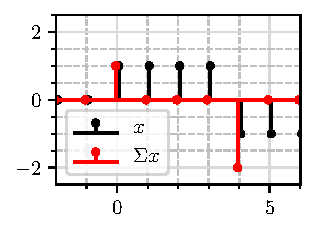
\includegraphics[scale=1]{fig/crtaj_dt_a.pdf}
        \caption{}
    \end{subfigure}
    \hspace*{0pt}\hfill
    \begin{subfigure}[c]{0.45\textwidth}
        \centering
        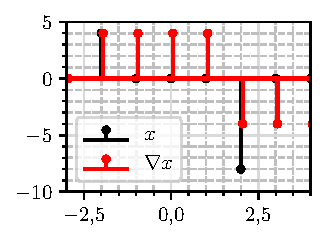
\includegraphics[scale=1]{fig/crtaj_dt_b.pdf}
        \caption{}
    \end{subfigure}
    \hfill
    \hspace*{0pt}

    \hspace*{0pt}\hfill
    \begin{subfigure}[c]{0.45\textwidth}
        \centering
        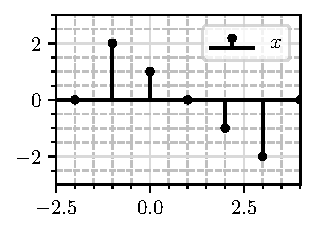
\includegraphics[scale=1]{fig/crtaj_dt_v.pdf}
        \caption{}
    \end{subfigure}
    \hspace*{0pt}\hfill
    \begin{subfigure}[c]{0.45\textwidth}
        \centering
        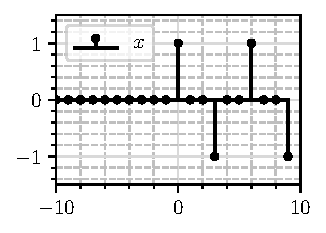
\includegraphics[scale=1]{fig/crtaj_dt_d.pdf}
        \caption{}
    \end{subfigure}
    \hfill
    \hspace*{0pt}
    \caption{Уз задатак \ID. На апсциси је $n$, а на ординати су означене величине.}
\end{figure}